\documentclass{article}[11pt]
%Required: You must have these
\usepackage{graphicx}
\usepackage{tabularx}
\usepackage{natbib}

\usepackage{array}
\usepackage{amsmath}
%\usepackage[backend=bibtex]{biblatex}
\setkeys{Gin}{width=0.8\textwidth}
%\setlength{\captionmargin}{30pt}
\setlength{\abovecaptionskip}{10pt}
\setlength{\belowcaptionskip}{10pt}
\topmargin -1.5cm 
\oddsidemargin -0.04cm 
\evensidemargin -0.04cm 
\textwidth 16.59cm
\textheight 23.94cm 
\parskip 7.2pt 
\renewcommand{\baselinestretch}{1} 	
\parindent 0pt

\bibliographystyle{refs/styles/newphyto.bst}
\renewcommand{\thetable}{S\arabic{table}}
\renewcommand{\thefigure}{S\arabic{figure}}
%\usepackage{xr}
\usepackage{hyperref}
\usepackage{xr-hyper}
%\usepackage{hyperref}
\externaldocument{phen_framing}

\usepackage{Sweave}
\begin{document}
\Sconcordance{concordance:supple.tex:supple.Rnw:1 31 1 1 0 60 1}


\section{Tables}
\begin{table}[ht]
\centering

\label{listSp}
\begin{tabular}{lrr}
  \hline
Species & functional group & n \\ 
  \hline
  \emph{Acer pensylvanicum} & tree  & 2 \\ 
  *\emph{Acer spicatum} & tree & \emph{NA}  \\ 
   \emph{Alnus incana} & shrub & 31 \\ 
   \emph{Amelanchier canadensis} &  shrub & 6  \\ 
  \emph{Aronia melanocarpa} & shrub & 12 \\ 
  \emph{Betula alleghaniensis} &  tree & 24\\ 
  \emph{Betula papyrifera} &   tree & 13 \\ 
  \emph{Betula populifolia} &  tree & 24\\ 
  \emph{Diervilla lonicera} &  shrub  & 16 \\ 
  \emph{Myrica gale} &  shrub & 15\\ 
  *\emph{Quercus alba} &  tree & \emph{NA}\\ 
  *\emph{Quercus rubra} &  tree & \emph{NA}\\ 
  \emph{Sambucus racemosa} &  shrub & 11\\ 
  \emph{Sorbus americana} &  shrub & 5\\
  \emph{Spiraea alba} &  shrub & 19\\ 
  \emph{Spiraea tomentosa} &   shrub & 21 \\ 
 * \emph{Vaccinium myrtilloides} &  shrub & \emph{NA}\\ 
  \emph{Viburnum cassinoides} &  shrub & 25 \\ 
  \end{tabular}
  \caption{Common garden focal species. In 2017, olantings were randomized between 16 plot blocks. Individuals that were too small to survive outside were maintained in the growth facilities for an additional year and out-planted in the early spring of 2018. Plots were divided between tree plots which included species  \textit{Acer pensylvanicum}, \textit{Amelanchier canadensis}, \textit{Alnus incana}, \textit{Betula papyrifera}, \textit{Betula populifolia}, \textit{Beluta alleghaniensis}, \textit{Quercus alba}, and \textit{Quercus rubra} and shrub plots which included the remaining species and shade cloth. * indicates species that were planted but not included in analyses due to low survivorship.} 
\end{table}



\section{Figures}
 \begin{figure}[h!]
    \centering
 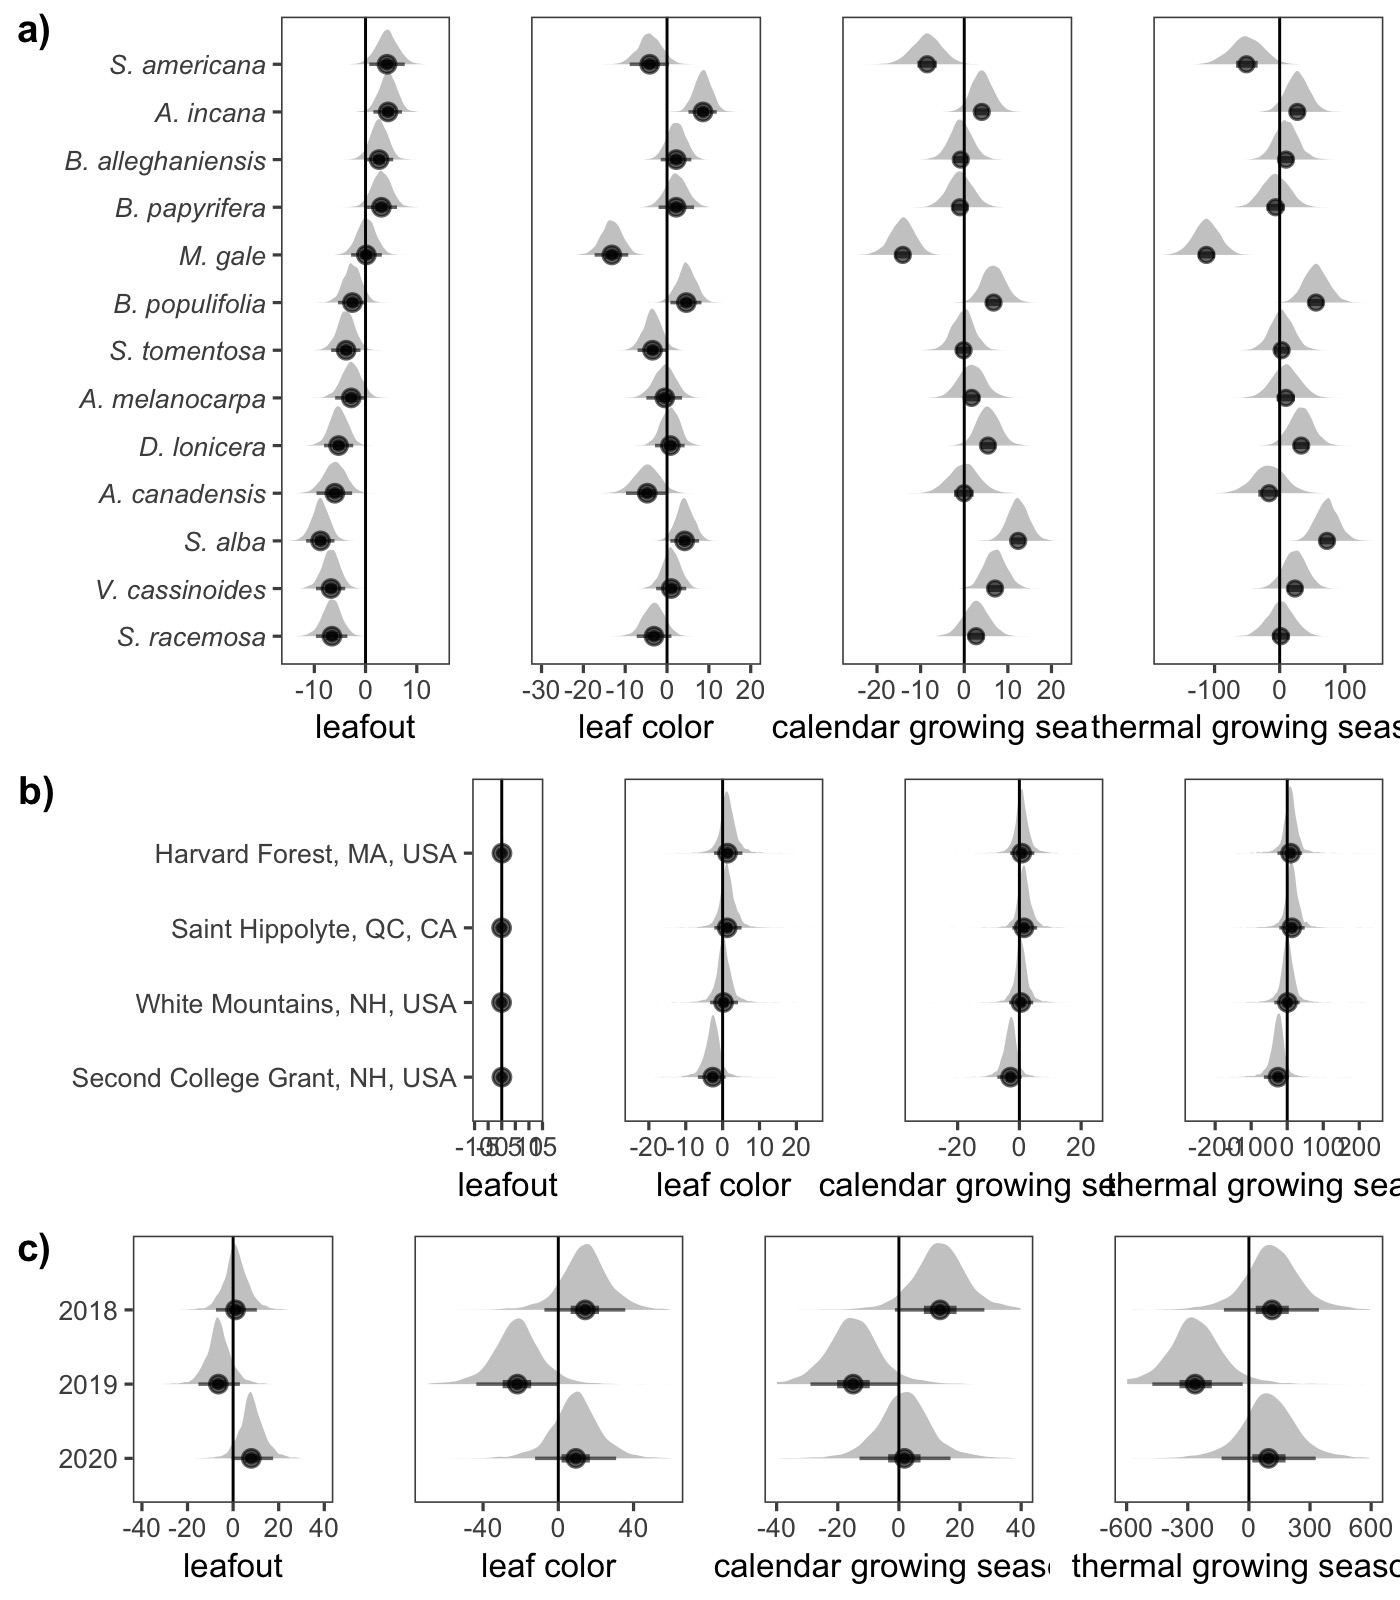
\includegraphics[width=.8\textwidth]{..//analyses/figures/full_var_parts.jpeg}
    \caption{Difference in leafout, leaf coloration and growing season length partitioned between species (a) populations (b) and years (c). Point represent the median effect size estimate, and bars the 50\% uncertainty intervals. The grey distribution depict the full uncertainty estimate around the estimate.}
    \label{fig:alta}
\end{figure}


\begin{figure}[h!]
    \centering
 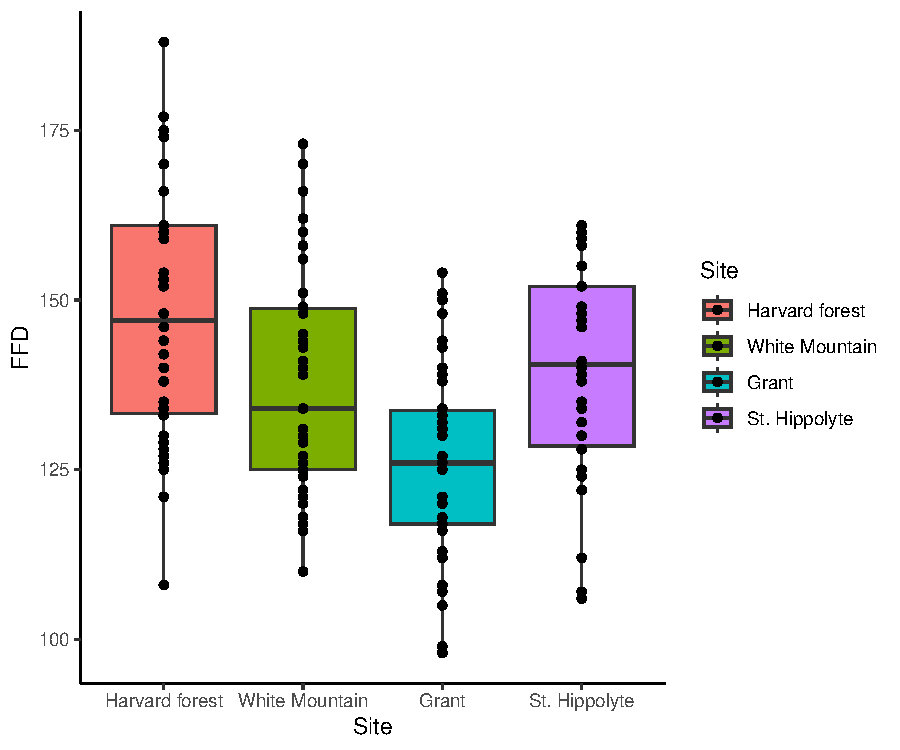
\includegraphics[width=.7\textwidth]{..//analyses/figures/ffdBySite.pdf}
    \caption{Frost free days! Deirdre can you fill in the caption about?}
    \label{fig:ffd}
\end{figure}


\begin{figure}[h!]
    \centering
 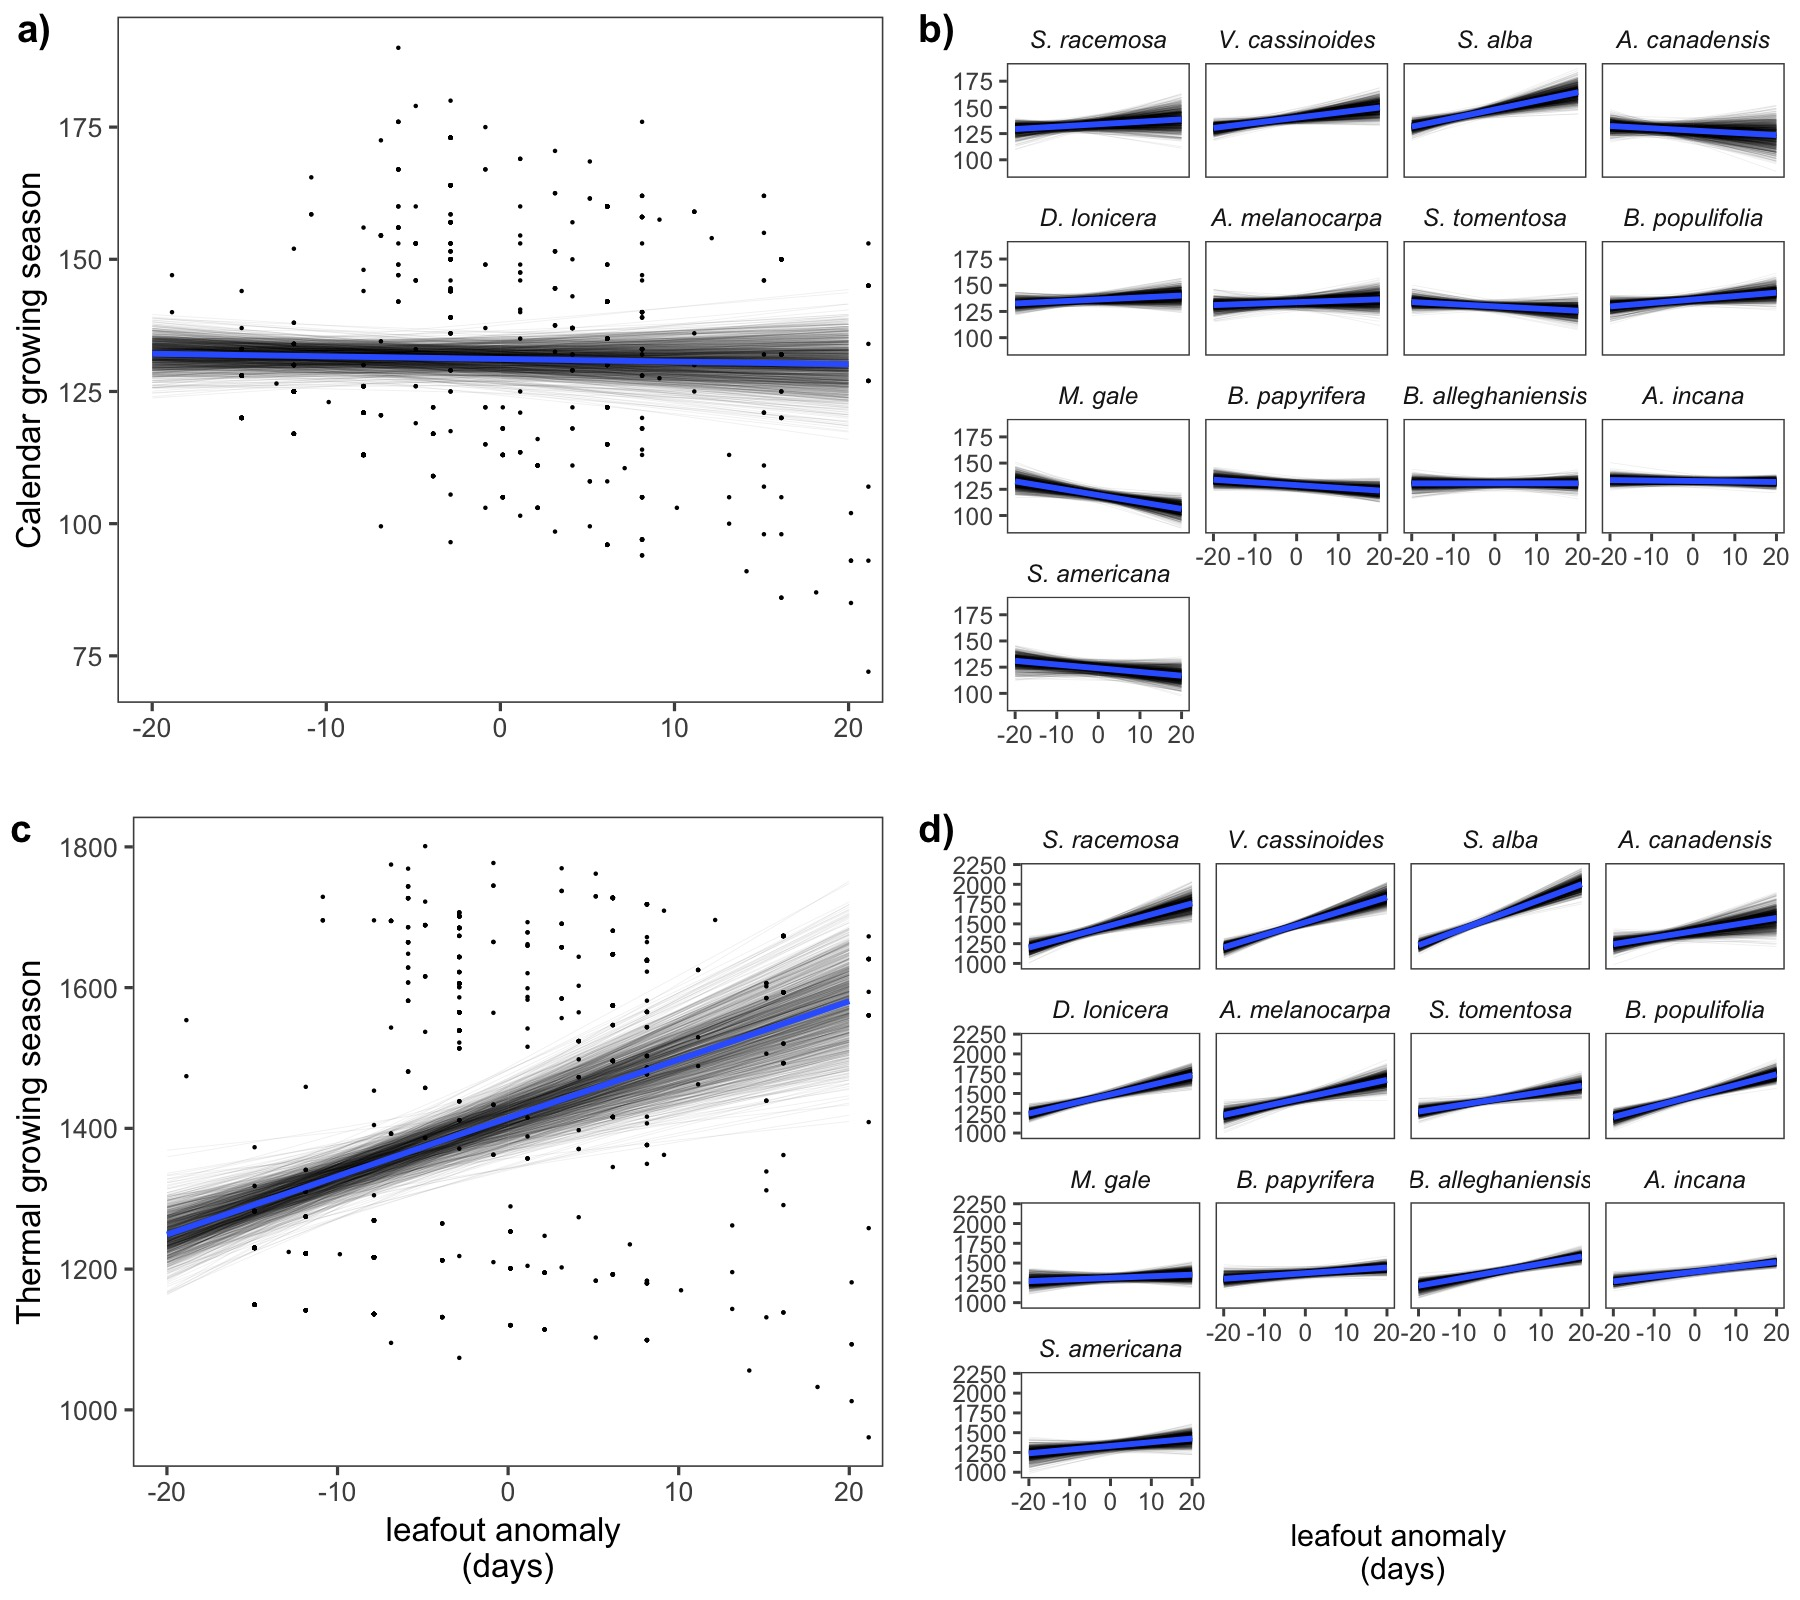
\includegraphics[width=.8\textwidth]{..//analyses/figures/fullgrowingseason_modplots.jpeg} 
    \caption{The relationship between Start of Spring (calendar day of leafout) and growing season length (defined by leaf coloration) differs between the calendar growing season and the thermal growing season. Later leafout did not affect calendar growing season (a) but this pattern varied  across species in our study (b). Increasingly later leafout resulted in a longer thermal growing season (c) though this effect was stronger for species that typically leafout earlier in the season---panels in c) display in the typical order of leafout among species. The blue trend lines represent the mean effect of leafout timing on growing season length and black lines represent 1000 draws from the posterior distribution as a measure of uncertainty. Points in a), and c) represent the raw data.}
    \label{fig:leafrel}
\end{figure}

\end{document}
